%\lstset{style=sqlstyle}

%CHAPTER
\chapter{Ověření efektivního vytěžování}
K ověření efektivního vytěžování bylo připraveno několik scénářů jak pro SQL, tak i pro Mongo + ElasticSearch.\newline
Napsat referenční stroj na kterém se testovalo - CPU, RAM, ...\todo{todo}
\section{Mongo + ElasticSearch}
\section{MySQL}
Pro MySQL bylo připraveno 10 scénářů, které testují všechny vytvořené tabulky v databázi. Každý scénář obsahuje textový popis, SQL příkaz, rychlost vykonání příkazu a ukázku výsledků.

\subsection{Scénář č.1}
\textbf{Textový popis}: Pět nejčastěji patentujících institucí v Izraeli v roce 2015
\newline
\textbf{SQL}: 
\begin{lstlisting}[language=SQL, breaklines=true, frame=single, label = {lst:elements_a}, captionpos=b]
select count(*), inventors.inventor from inventors left outer join patents on inventors.id_patent = patents.id where YEAR(patents.patent_date) = 2015 and patents.patent_id like '%IL%' group by inventors.inventor order by count(*) desc LIMIT 5;
\end{lstlisting}
\textbf{Rychlost vykonání dotazu}: \todo{TODO}
\newline
\textbf{Výsledek dotazu}:
\begin{figure}[h!]
\centering
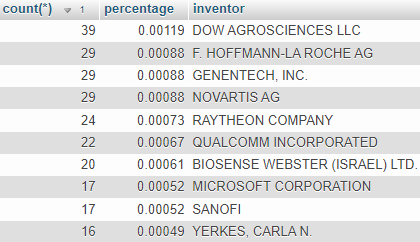
\includegraphics[width=8cm]{img/scenare/scenar_1}
\caption{Ukázka výsledku dotazu pro scénář č.1}
\label{fig:scenar1}
\end{figure}


\subsection{Scénář č.2}
\textbf{Textový popis}: Tři nejméně patentované obory v Kanadě od roku 2010
\newline
\textbf{SQL}: 
\begin{lstlisting}[language=SQL, breaklines=true, frame=single, label = {lst:elements_a}, captionpos=b]
select count(*), classification.section from classification left outer join patents on patents.id = classification.id_patent where YEAR(patents.patent_date) >= 2010 and patents.patent_id like '%CA%' group by classification.section order by count(*) asc LIMIT 3;
\end{lstlisting}
\textbf{Rychlost vykonání dotazu}: \todo{TODO}
\newline
\textbf{Výsledek dotazu}:\todo{TODO}
\begin{figure}[h!]
\centering
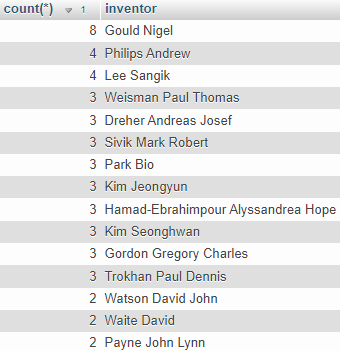
\includegraphics[width=6cm]{img/scenare/scenar_9}
\caption{Ukázka výsledku dotazu pro scénář č.2}
\label{fig:scenar2}
\end{figure}

\subsection{Scénář č.3}
\textbf{Textový popis}: Nejčastější klasifikace patentu za rok 2008 ve Španělsku
\newline
\textbf{SQL}: 
\begin{lstlisting}[language=SQL, breaklines=true, frame=single, label = {lst:elements_a}, captionpos=b]
select count(*), classification.section, classification.class, classification.subclass from classification left outer join patents on patents.id = classification.id_patent where YEAR(patents.patent_date) = 2008 and patents.patent_id LIKE '%ES%' group by classification.section, classification.class, classification.subclass order by count(*) desc LIMIT 1;
\end{lstlisting}
\textbf{Rychlost vykonání dotazu}: \todo{TODO}
\newline
\textbf{Výsledek dotazu}:
\begin{figure}[h!]
\centering
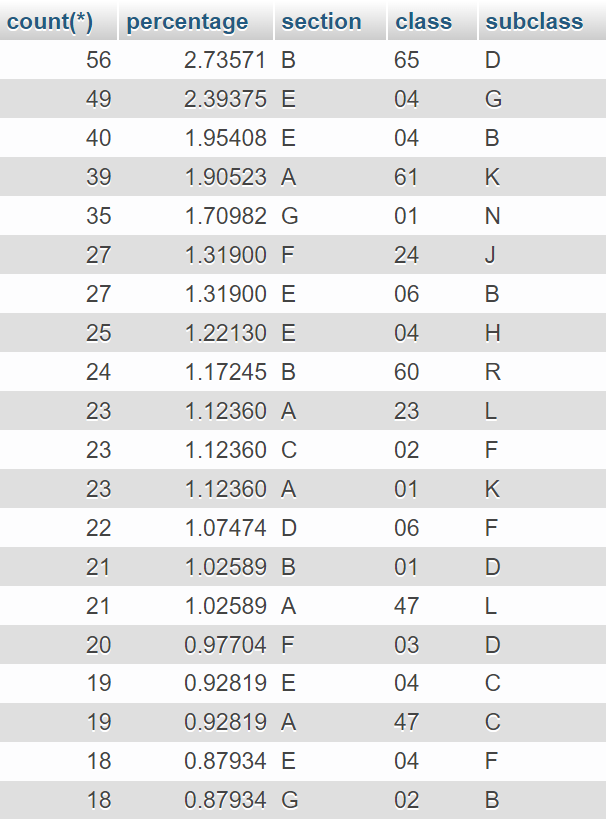
\includegraphics[width=8cm]{img/scenare/scenar_3}
\caption{Ukázka výsledku dotazu pro scénář č.3}
\label{fig:scenar3}
\end{figure}

\subsection{Scénář č.4}
\textbf{Textový popis}: Autor s největším počtem patentů ze všech zemí
\newline
\textbf{SQL}: 
\begin{lstlisting}[language=SQL, breaklines=true, frame=single, label = {lst:elements_a}, captionpos=b]
select count(*), inventors.inventor from inventors left outer join patents on patents.id = inventors.id_patent group by inventors.inventor order by count(*) desc LIMIT 1;
\end{lstlisting}
\textbf{Rychlost vykonání dotazu}: \todo{TODO}
\newline
\textbf{Výsledek dotazu}:\todo{TODO}
\begin{figure}[h!]
\centering
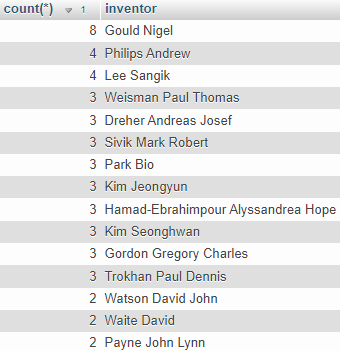
\includegraphics[width=6cm]{img/scenare/scenar_9}
\caption{Ukázka výsledku dotazu pro scénář č.4}
\label{fig:scenar4}
\end{figure}

\subsection{Scénář č.5}
\textbf{Textový popis}: Nejméně používaný jazyk pro patenty za rok 2003
\newline
\textbf{SQL}: 
\begin{lstlisting}[language=SQL, breaklines=true, frame=single, label = {lst:elements_a}, captionpos=b]
select count(*), patents.language from patents where patents.language not like '%-%' group by patents.language order by count(*) asc LIMIT 1;
\end{lstlisting}
\textbf{Rychlost vykonání dotazu}: \todo{TODO}
\newline
\textbf{Výsledek dotazu}:\todo{TODO}
\begin{figure}[h!]
\centering
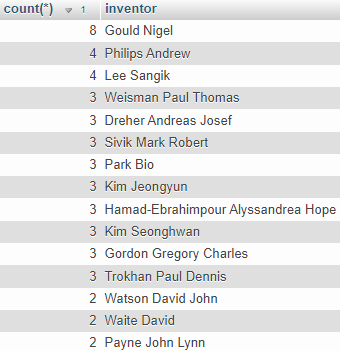
\includegraphics[width=6cm]{img/scenare/scenar_9}
\caption{Ukázka výsledku dotazu pro scénář č.5}
\label{fig:scenar5}
\end{figure}

\subsection{Scénář č.6}
\textbf{Textový popis}: Deset Institucí / autorů s patenty pokrývající největší množství oborů
\newline
\textbf{SQL}: 
\begin{lstlisting}[language=SQL, breaklines=true, frame=single, label = {lst:elements_a}, captionpos=b]
select count(distinct classification.section), inventors.inventor from inventors left outer join classification on classification.id_patent = inventors.id_patent where section is not null group by inventors.inventor order by count(distinct classification.section) desc LIMIT 10;
\end{lstlisting}
\textbf{Rychlost vykonání dotazu}: \todo{TODO}
\newline
\textbf{Výsledek dotazu}:\todo{TODO}
\begin{figure}[h!]
\centering
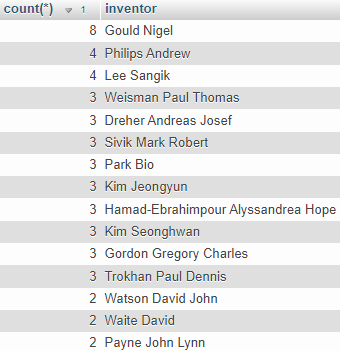
\includegraphics[width=6cm]{img/scenare/scenar_9}
\caption{Ukázka výsledku dotazu pro scénář č.6}
\label{fig:scenar6}
\end{figure}

\subsection{Scénář č.7}
\textbf{Textový popis}: Země s nejvíce patenty od roku 2018
\newline
\textbf{SQL}: 
\begin{lstlisting}[language=SQL, breaklines=true, frame=single, label = {lst:elements_a}, captionpos=b]
select count(*), patents.country from patents where YEAR(patents.patent_date) >= 2018 group by patents.country order by count(*) desc;
\end{lstlisting}
\textbf{Rychlost vykonání dotazu}: \todo{TODO}
\newline
\textbf{Výsledek dotazu}:\todo{TODO}
\begin{figure}[h!]
\centering
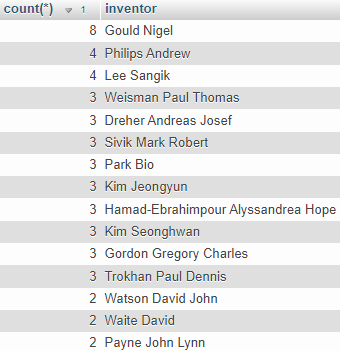
\includegraphics[width=6cm]{img/scenare/scenar_9}
\caption{Ukázka výsledku dotazu pro scénář č.7}
\label{fig:scenar7}
\end{figure}

\subsection{Scénář č.8}
\textbf{Textový popis}: Nejvíce používaný jazyk pro patenty ve Francii
\newline
\textbf{SQL}: 
\begin{lstlisting}[language=SQL, breaklines=true, frame=single, label = {lst:elements_a}, captionpos=b]
select count(*), patents.language from patents where patents.patent_id like '%FR%' group by patents.language order by count(*) desc;
\end{lstlisting}
\textbf{Rychlost vykonání dotazu}: \todo{TODO}
\newline
\textbf{Výsledek dotazu}:\todo{TODO}
\begin{figure}[h!]
\centering
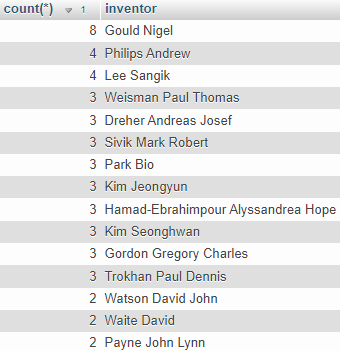
\includegraphics[width=6cm]{img/scenare/scenar_9}
\caption{Ukázka výsledku dotazu pro scénář č.8}
\label{fig:scenar8}
\end{figure}

\subsection{Scénář č.9}
\textbf{Textový popis}: Tři nejčastěji patentující instituce / autoři v Anglii v textilním oboru za rok 2013
\newline
\textbf{SQL}: 
\begin{lstlisting}[language=SQL, breaklines=true, frame=single, label = {lst:elements_a}, captionpos=b]
select count(*), inventors.inventor from inventors left outer join patents on patents.id = inventors.id_patent left outer join classification on classification.id_patent = patents.id where classification.section like '%D%' and patents.patent_id like '%GB%' and YEAR(patents.patent_date) = 2013 group by inventors.inventor order by count(*) desc LIMIT 3
\end{lstlisting}
\textbf{Rychlost vykonání dotazu}: \todo{TODO}
\newline
\textbf{Výsledek dotazu}:
\begin{figure}[h!]
\centering
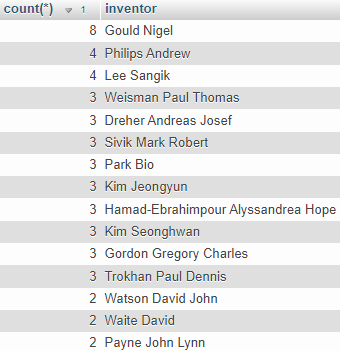
\includegraphics[width=6cm]{img/scenare/scenar_9}
\caption{Ukázka výsledku dotazu pro scénář č.9}
\label{fig:scenar9}
\end{figure}